\subsection{Leibniz: Infinitesimals, Harmony, and the Algebra of Change}

While Newton conceived calculus through the lens of motion and absolute time, \textbf{Gottfried Wilhelm Leibniz} envisioned something different:  
A symbolic language of relations, a grammar for understanding the infinitesimal structure of change itself.

For Leibniz, mathematics was not merely a description of physical motion; it was a reflection of divine rationality—the unfolding of a universe optimized through the simplest possible laws.





\subsection{A Symbolic View of Calculus}

Where Newton defined fluxions as rates of physical change flowing through absolute time, Leibniz defined 
differentials as symbolic quantities: infinitely small changes, whose ratios revealed the hidden structure of 
curves, motions, and forces.

He introduced the notation:

\[
\frac{dy}{dx}
\]

—an abstract ratio of infinitesimal differences. Unlike Newton’s fluxions, which were anchored to real-world time, 
Leibniz's differentials existed independently, manipulated through symbolic rules.

At the heart of Leibniz’s vision was the idea that:

\begin{itemize}
    \item \( dx \) is an infinitesimal change in the input.
    \item \( dy \) is the corresponding infinitesimal change in the output.
    \item Their ratio \( \frac{dy}{dx} \) captures the local behavior of a function at a point.
\end{itemize}

\begin{HistoricalSidebar}{Leibniz’s Notation vs Newton’s Fluxions}

  Where Newton viewed calculus as describing motion through absolute time, Leibniz saw it as a symbolic algebra of infinitesimal relations.

  \medskip

  Newton's fluxions (\( \dot{x} \)) depended on the notion of a cosmic timekeeper—an invisible river against which change was measured.

  \medskip

  Leibniz’s differentials (\( dx, dy \)) needed no such clock. They were purely algebraic, describing how quantities changed in relation to each other, without reference to any external temporal flow.

  \medskip

  Today, calculus textbooks overwhelmingly use Leibniz’s notation—not because Newton was wrong, but because Leibniz’s abstraction made the machinery of change universally portable.

\end{HistoricalSidebar}





\subsection{Leibniz’s Infinitesimals: Bridging the Finite and the Infinite}

In Leibniz’s mind, infinitesimals were not imaginary fictions—they were real mathematical entities that bridged the gap between finite and infinite quantities. He imagined curves not as smooth wholes, but as stitched together from infinitely many infinitesimal linear segments. Zoom close enough, and any curve would look like a straight line.

Thus, differentiation became the study of these infinitesimal triangles.  He expressed this beautifully:
\[
dy = v\,dt
\quad \text{and} \quad
v = \frac{ds}{dt}
\]
For Leibniz, the world was a seamless fabric of change woven from vanishing threads.

While he did not explicitly use the term “factorization” in the modern sense, he nonetheless employed techniques that anticipate the analysis of functions such as quadratics.  In classical algebra one finds the minimum of a quadratic by rewriting

\[
f(x) = ax^2 + bx + c
\quad\longrightarrow\quad
a\bigl(x + \tfrac{b}{2a}\bigr)^2 - \frac{b^2}{4a} + c,
\]

but Leibniz’s approach relied instead on infinitesimal changes.  He recognized that the critical points of \(f(x)\) occur where its differential vanishes:

\[
df = \frac{d}{dx}(ax^2 + bx + c)\,dx = (2ax + b)\,dx = 0.
\]

Setting \(2ax + b = 0\) yields \(x = -\tfrac{b}{2a}\), the same location of the quadratic’s minimum.  In this way, Leibniz’s theory of differentials—by focusing on vanishing infinitesimals—provided a unified method for locating minima and maxima without recourse to factorization, revealing the power of his new calculus to probe the very slopes and turning points of curves.


Leibniz’s algebraic calculus turns the mechanics of differentiation into simple symbol manipulations.  At its core lies the product rule:

\[
d(u\,v)
\;=\;
u\,d v \;+\; v\,d u,
\]

which immediately yields the familiar derivative formula

\[
\frac{d}{dx}\bigl(u(x)\,v(x)\bigr)
\;=\;
u(x)\,\frac{dv}{dx} \;+\; v(x)\,\frac{du}{dx}.
\]

\bigskip

\textbf{Why algebraic?}  Unlike Newton’s geometric fluxions—where one imagines infinitesimal “velocities” sweeping out areas—Leibniz’s rule requires no picture of moving points or polygons.  The differential operator \(d\) is treated like an algebraic symbol with two simple properties:

\begin{itemize}
  \item \emph{Linearity:} \(d(u + v) = du + dv\).
  \item \emph{Product rule:} \(d(u\,v) = u\,dv + v\,du\).
\end{itemize}

Leibniz’s algebraic rules for \(d\) follow naturally from his conception of differentials as infinitesimal increments.


\textbf{Linearity.}  By definition, if \(u\) and \(v\) are two functions of \(x\), then their differentials arise from infinitesimal changes:

\[
du = u(x + dx) - u(x), 
\quad
dv = v(x + dx) - v(x).
\]

Hence for the sum \(u + v\),

\[
d(u+v)
= (u + v)(x + dx) - (u + v)(x)
= \bigl[u(x+dx) - u(x)\bigr] \;+\; \bigl[v(x+dx) - v(x)\bigr]
= du + dv.
\]

\textbf{Product Rule.}  Consider the product \(u\,v\).  Expanding the increment,
\[
d(u\,v)
= u(x+dx)\,v(x+dx) \;-\; u(x)\,v(x).
\]

Write \(u(x+dx)=u+du\) and \(v(x+dx)=v+dv\).  Then

\[
d(u\,v)
= (u + du)(v + dv) - u v
= u\,dv + v\,du + du\,dv.
\]

Since \(du\) and \(dv\) are both infinitesimal, the product \(du\, dv\) is a “second-order” 
infinitesimal—negligible compared to the first-order terms.  Discarding \(du\, dv\) yields

\[
d(u\,v) = u\,dv + v\,du,
\]

exactly Leibniz’s product rule.



\subsubsection*{Concrete Examples of Linearity and the Product Rule}

To see why these rules matter, consider simple choices for \(u(x)\) and \(v(x)\):

\paragraph{1. Linearity of \(d\).}  
Let
\[
u(x) = x^2,
\quad
v(x) = 3x.
\]
Then
\[
du = d(x^2) = 2x\,dx,
\qquad
dv = d(3x) = 3\,dx.
\]
Their sum \(u+v = x^2 + 3x\) has differential
\[
d(u+v)
= d\bigl(x^2 + 3x\bigr)
= d(x^2) + d(3x)
= 2x\,dx + 3\,dx
= du + dv.
\]
Thus, differentiating the sum is the same as summing the differentials.

\paragraph{2. The Product Rule.}  

Let

\[
u(x) = x^2,
\quad
v(x) = \sin x.
\]

Compute

\[
du = d(x^2) = 2x\,dx,
\qquad
dv = d(\sin x) = \cos x\,dx.
\]

Their product \(u\,v = x^2\sin x\) has differential

\[
d(u\,v)
= d\bigl(x^2 \sin x\bigr)
= x^2\,d(\sin x) + \sin x\,d(x^2)
= x^2\cos x\,dx + \sin x\,(2x\,dx)
= \bigl(x^2\cos x + 2x\sin x\bigr)\,dx,
\]

exactly matching

\[
u\,dv + v\,du
= x^2(\cos x\,dx) + \sin x\,(2x\,dx).
\]

These examples show how—thanks to linearity—differentials split neatly over sums, and—thanks to the 
product rule—differentials of products capture each factor’s contribution in a single algebraic step, 
without any geometric constructions.  














Because these rules hold for any symbols \(u\) and \(v\), one can:

\begin{itemize}
  \item \emph{Compose:} derive the chain rule \(d\bigl(f(g)\bigr)=f'(g)\,dg\) by treating \(dg\) as a new symbol.
  \item \emph{Iterate:} obtain the \(n\)th derivative of a product via the Leibniz rule 
    \[
      d^n(u\,v)
      = \sum_{k=0}^n \binom{n}{k}\,d^k u \;d^{\,n-k}v.
    \]
  \item \emph{Invert:} rearrange to get integration by parts directly:
    \[
      \int u\,dv = u\,v - \int v\,du.
    \]
\end{itemize}

This purely algebraic framework makes calculus universally portable—applicable to functions, power series, 
differential forms, and even non‐commutative operators—without reliance on any geometric or physical intuition.  
Leibniz’s symbolic method thus unlocked the full power of differential and integral calculus as an algebraic art.  




\subsection{Integration: Recombining Infinitesimal Threads into Wholes}

If differentiation tore curves into their infinitesimal triangles, integration wove them back into unity.  
Leibniz introduced the symbol \(\displaystyle \int\) --- an elongated ``S'' for \emph{summa} --- to represent 
the accumulation of infinitely many infinitesimal parallelograms \(f(x)\,dx\).  In his own notation he might write:

\[
\int f(x)\,dx
=
f(x_{1})\,dx + f(x_{2})\,dx + f(x_{3})\,dx + \cdots,
\]
each term \(f(x_{i})\,dx\) standing for one infinitesimal parallelogram.  

\medskip

\begin{figure}[H]
  \centering
  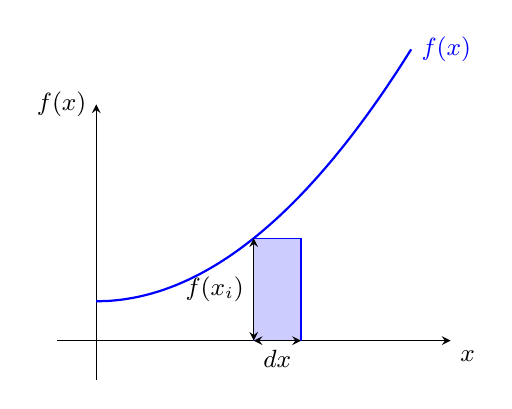
\begin{tikzpicture}[scale=1, every node/.style={font=\small}, >=stealth]
    % Parameters
    \def\a{0}         % left end of interval
    \def\b{4}         % right end of interval
    \def\xi{2}        % sample point x_i
    \def\dx{0.6}      % width dx

    % Axes
    \draw[->] (\a-0.5,0) -- (\b+0.5,0) node[below right] {$x$};
    \draw[->] (0,-0.5) -- (0,3) node[left] {$f(x)$};

    % The curve f(x)
    \draw[domain=\a:\b,smooth,variable=\x,thick,blue]
      plot ({\x},{0.2*(\x)^2 + 0.5}) node[right] {$f(x)$};

    % Compute f(x_i)
    \pgfmathsetmacro{\yi}{0.2*(\xi)^2 + 0.5}

    % Coordinates of the infinitesimal parallelogram
    \coordinate (A) at (\xi,       0);
    \coordinate (B) at (\xi,       \yi);
    \coordinate (C) at ({\xi+\dx}, \yi);
    \coordinate (D) at ({\xi+\dx}, 0);

    % Shade the parallelogram f(x_i) dx
    \filldraw[fill=blue!20, draw=blue] (A) -- (B) -- (C) -- (D) -- cycle;

    % Labels for dx and f(x_i)
    \draw[<->] (A) -- node[below] {$dx$} (D);
    \draw[<->] (A) -- node[left] {$f(x_i)$} (B);
  \end{tikzpicture}
  \caption{An infinitesimal parallelogram $f(x_i)\,dx$ illustrating Leibniz’s integration as the sum of vanishing threads.}
  \label{fig:leibniz-integration}
\end{figure}

\medskip


Integration thus reverses differentiation:
\[
y - y_{0}
=
\int v\,dt,
\]
signifying that the total change \(y - y_{0}\) arises by summing all the vanishing contributions \(v\,dt\).  
Whether one computes the area under a curve, the distance traveled from a velocity law, or the work done by 
a force, integration unites the vanished threads into a continuous whole—restoring the seamless fabric of 
geometry and motion.

\begin{figure}[H]
  \centering
  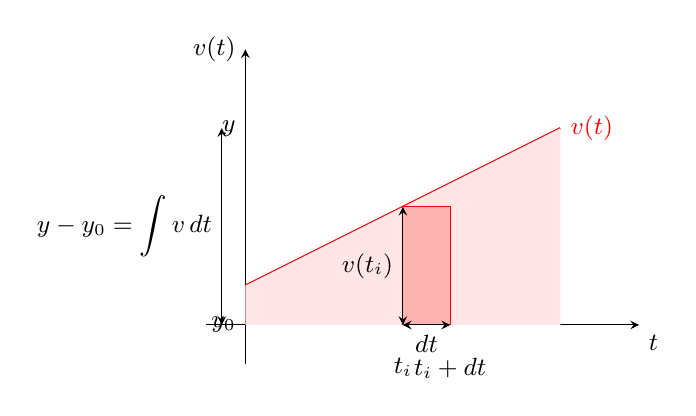
\begin{tikzpicture}[scale=1, every node/.style={font=\small}, >=stealth]
    % Parameters
    \def\tzero{0}       % start time
    \def\T{4}           % end time
    \def\ti{2}          % sample point t_i
    \def\dt{0.6}        % width dt

    % Axes for velocity
    \draw[->] (\tzero-0.5,0) -- (\T+1,0) node[below right] {$t$};
    \draw[->] (0,-0.5) -- (0,3.5) node[left] {$v(t)$};

    % Velocity curve v(t) = 0.5 t + 0.5
    \draw[domain=\tzero:\T,smooth,variable=\t,thick,red]
      plot ({\t},{0.5*\t + 0.5}) node[right] {$v(t)$};

    % Shade the total area under the curve (schematic)
    \fill[red!10]
      plot[domain=\tzero:\T] (\x,{0.5*\x + 0.5}) -- (\T,0) -- (\tzero,0) -- cycle;

    % Compute v(t_i)
    \pgfmathsetmacro{\vi}{0.5*\ti + 0.5}

    % Coordinates of the infinitesimal parallelogram
    \coordinate (P) at (\ti,      \vi);
    \coordinate (Q) at ({\ti+\dt},\vi);
    \coordinate (R) at ({\ti+\dt},0);
    \coordinate (S) at (\ti,      0);

    % Shade the infinitesimal parallelogram v(t_i) dt
    \filldraw[fill=red!30,draw=red] (P) -- (Q) -- (R) -- (S) -- cycle;

    % Labels for dt and v(t_i)
    \draw[<->] (S) -- node[below] {$dt$} (R);
    \draw[<->] (S) -- node[left]  {$v(t_i)$} (P);

    % Mark t_i and t_i + dt
    \node[below] at (\ti, -0.3)           {$t_i$};
    \node[below] at ({\ti+\dt}, -0.3)    {$t_i + dt$};

    % Displacement axis and horizontal equation label
    \draw[<->] (-0.3,0) -- (-0.3,2.5) node[midway,left] {$y - y_{0} = \displaystyle\int v\,dt$};

    % Mark y_0 and y on the vertical axis
    \node[left]  at (0,0)    {$y_0$};
    \node[left]  at (0,2.5)  {$y$};
  \end{tikzpicture}
  \caption{Summing all the infinitesimal parallelograms $v(t_i)\,dt$ from $t_0$ to $t$ yields the total displacement $y - y_0$.}
  \label{fig:leibniz-integration-annotated-horizontal}
\end{figure}



\subsection{Integration by Parts and the Leibniz Rule: An Algebraic Perspective}

Leibniz’s differential calculus yields a purely algebraic route to integration by parts and the general Leibniz rule for products—distinct from Newton’s geometric fluxional constructions.

\medskip

\noindent\textbf{Integration by Parts.}  From the product‐rule differential
\[
d(u\,v) \;=\; u\,dv + v\,du,
\]
one simply “sums” (integrates) both sides:
\[
\int d(u\,v)
\;=\;
\int u\,dv \;+\; \int v\,du.
\]
Since \(\displaystyle \int d(u\,v)=u\,v\), Leibniz’s notation immediately gives
\[
u\,v \;=\; \int u\,dv \;+\; \int v\,du
\quad\Longrightarrow\quad
\int u\,dv = u\,v - \int v\,du.
\]
No geometric areas or fluxional polygons are needed—just the algebra of differentials and the symbol \(\int\).

\medskip

\noindent\textbf{The Leibniz Rule.}  Leibniz also formulated the rule for the \(n\)th differential of a product:
\[
d^n(u\,v)
\;=\;
\sum_{k=0}^{n} \binom{n}{k}\,d^k u \;\;d^{\,n-k}v.
\]
Viewed algebraically, this is nothing more than iterating the linearity and product‐rule properties of \(d\).  One then integrates term by term when needed, or uses these combinatorial coefficients directly in series expansions, without invoking any geometric underpinning.

\medskip

Thus, in Leibniz’s hands the core operations of “integration by parts” and the “Leibniz rule” emerge from straightforward algebraic manipulations of his differential symbols—whereas Newton’s original approach appealed to geometric arguments about fluxions and areas under moving loci.  Leibniz’s method paved the way for later developments in operator calculus and symbolic manipulation.  


\begin{HistoricalSidebar}{From Leibniz’s Differentials to Euler’s Function Notation}

  Leibniz’s genius was to treat differentials as algebraic infinitesimals. He wrote 

  \[
  \frac{dy}{dx},\quad d^2y,\quad \int f(x)\,dx,
  \]

  with an implicit understanding that \(y\) was “the” dependent quantity.  His notation emphasized the
  process of differentiation and integration as manipulations of vanished quantities, but left the 
   notion of a function itself somewhat abstract.

  \medskip
  
  By the mid-18th century, Euler had introduced explicit function notation and streamlined derivative symbols:

  \[
  f(x), \quad y = f(x), \quad f'(x), \quad f''(x), \quad f^{(n)}(x).
  \]

  He also popularized the notation

  \[
  \sum_{k=0}^n a_k x^k,\quad e^x,\quad \sin x,\quad \cos x,
  \]

  making both series and transcendental functions part of the same formal language.  Euler’s use of parentheses 
  to show the argument of a function and the prime‐mark for derivatives laid the foundation for the 
  notation we still use today.

  \medskip
  
  In modern calculus we thus combine Leibniz’s differential symbol \(d\) and integral sign \(\int\) with Euler’s 
  function-and-prime notation:

  \[
  \int_a^b f(x)\,dx,\quad f'(x),\quad f^{(n)}(x).
  \]

  This hybrid system retains the algebraic clarity of Leibniz’s infinitesimals while leveraging Euler’s emphasis 
  on functions as objects of study.
\end{HistoricalSidebar}


\subsection{Why “Differential” Calculus?}

The term “differential” calculus arises directly from Leibniz’s emphasis on the infinitesimal change—or \emph{differential}—as the fundamental building block of his theory.  In his view, every curve, motion, or varying quantity could be understood by probing how a vanishingly small increment in the input (\(dx\)) produces a corresponding increment in the output (\(dy\)).  By focusing on these “differentials” themselves, Leibniz elevated the act of computing ratios of little changes to the central operation of calculus.

\medskip

\noindent\textbf{Key ideas behind the name:}
\begin{itemize}
  \item \emph{Local Linearization.}  Each differential pair \((dx,\,dy)\) captures the local linear approximation to a curve.  Rather than treating the whole function globally, one studies it slice by slice in terms of these infinitesimal threads.
  \item \emph{Algebraic Manipulation.}  Differentials behave like algebraic symbols—one can add, multiply, and even divide them—allowing one to derive general rules (product rule, chain rule) by purely symbolic means.
  \item \emph{Reversibility.}  Just as differentiation peels away an infinitesimal layer of the function, integration recombines the differentials into a whole.  The “forward” process of forming \(dy = f'(x)\,dx\) and the “inverse” process \(\int f(x)\,dx\) both revolve around the same differential symbol \(dx\).
\end{itemize}

Thus, what we call “differential calculus” is really the study of how infinitesimal variations propagate through functions—and how those tiny variations can be manipulated and summed to reveal both the instantaneous behavior and the global structure of curves, motions, and physical laws.  










\subsection{The Metaphysical Vision: Harmony and Optimization}

Leibniz's calculus was part of a much larger philosophical program.

He believed that God, being perfect, would create the \textbf{best of all possible worlds}: the simplest 
causes yielding the most complex and beautiful effects.

In this vision, nature operated according to \textbf{optimization principles}—minimizing effort, 
maximizing harmony. Change was rational, structured, elegant.

Calculus, in Leibniz's hands, was not just a mathematical tool. It was a theological insight, a 
window into the divine algorithm underlying reality.

\begin{HistoricalSidebar}{Leibniz—Calculus, Harmony, and the Divine Algorithm}
  
  \textbf{Gottfried Wilhelm Leibniz} didn’t just invent calculus—he invented it as part of a larger metaphysical project: to show that the universe itself was the optimal solution to a divine equation.

  For Leibniz, mathematics was philosophy in symbolic form.  
  His obsession with optimization—simple laws, rich outcomes—foreshadowed the later development of variational principles in physics.

  \medskip

  His differential notation (\( dx, dy \)) reflected this view: nature changes not by abrupt leaps, but by smooth, rational transitions—gliding through possibility space with divine efficiency.

  \medskip

  To Leibniz, every mathematical expression was a hint, a whisper of God's mind.

  \medskip

  \textbf{Quote from Leibniz (1686):}
  \begin{quote}
  The present is pregnant with the future; the future could be calculated from it, if we had sufficient knowledge of all causes.
  \end{quote}
  
\end{HistoricalSidebar}

\subsection{Contrast with Newton: Time vs Structure}

While Leibniz built a calculus of structure and relationship, Newton grounded his in absolute time and physical flux.

\begin{center}
\begin{tabular}{c|c}
\textbf{Newton (contrast)} & \textbf{Leibniz (focus)} \\
\hline
Fluxions: change over absolute time & Differentials: ratios of change \\
Geometry tied to physical motion & Algebra abstracted from motion \\
Divine time as universal backdrop & Divine optimization as structural law \\
Physical causality (force) & Structural relations (infinitesimals) \\
\end{tabular}
\end{center}

Newton’s calculus flowed with time; Leibniz’s calculus floated above it.

Both contributed essential tools to modern science, but it was Leibniz’s abstract, symbolic vision that made calculus portable—extending it beyond planets and physics to fields as diverse as economics, statistics, and machine learning.

\subsection{Leibniz’s Enduring Legacy}

Today, whenever we write:

\[
\frac{dy}{dx}
\quad \text{or} \quad
\int f(x)\,dx
\]

—whenever we study derivatives as relationships, or integrals as accumulated changes—we walk the road that Leibniz paved.

His calculus is not a description of physical flow, but a universal language of structured change.

Where Newton saw the river of time, Leibniz built the bridge of symbols.

\begin{tcolorbox}[colback=gray!5!white, colframe=black, title=\textbf{Philosophical Footnote: Einstein and the Reunion of Newton and Leibniz}, fonttitle=\bfseries, arc=1.5mm, boxrule=0.4pt]

  In the 20th century, \textbf{Albert Einstein} would confront a strange destiny: to reconcile the two divergent visions born in the calculus of Newton and Leibniz.

  \medskip
  
  Einstein’s theory of \textbf{relativity} demanded both:

  \medskip
  
  \begin{itemize}
      \item \textbf{Newton’s dynamical realism} — that change is real, physical, and law-governed.
      \item \textbf{Leibniz’s structural relationalism} — that space, time, and motion are not absolute stages, but networks of relationships between events.
  \end{itemize}

  \medskip
  
  When Einstein bent space and time into a single fabric, he inherited Newton’s faith in the objective structure of the universe—but stripped away Newton’s absolute time.  When he described motion as the geometry of spacetime itself, he realized Leibniz’s dream: that relations, not substances, are primary.
  
  \medskip
  
  In a way, relativity is where Newton’s flowing clock and Leibniz’s invisible algebra finally shook hands—two rival visions, fused into the strange, flexible, curved continuum we now call spacetime.
  
  \medskip
  
  \textbf{In the beginning, there was motion. In the end, there were relations.}

\end{tcolorbox}

\subsection{A New Kind of Equation: Relations of Change}

Leibniz didn’t just invent notation—he opened the door to a new kind of equation.

By symbolizing derivatives as \( \frac{dy}{dx} \), he made it possible to write \textbf{equations where the unknown wasn’t a number, but a function whose rate of change followed certain rules}. These became known as \textbf{differential equations}: equations that relate a function to its derivatives.

For Leibniz, differential equations were a natural extension of calculus. If differentiation measured change, and integration summed change, then a differential equation was a statement about how a quantity \emph{must change}—a recipe for motion, growth, or interaction.

This wasn’t just symbolic cleverness. It created a new mathematical language for describing the world. Forces, orbits, velocities, flows—anything changing over time or space could now be encoded as an equation involving derivatives.

Leibniz’s framework laid the foundation for later generations of mathematicians and physicists, who would turn these symbolic expressions into tools for solving real-world problems.

\vspace{1em}

\begin{center}
\textit{Leibniz gave calculus its grammar—and with it, a way to write the laws of change themselves.}
\end{center}
